\documentclass[11pt]{standalone}

\usepackage{lmodern}	% font definition
\usepackage{amsmath}	% math fonts
\usepackage{amsthm}
\usepackage{amsfonts}
\usepackage{pgfplots}

\usepackage{pgfplots}
\usepackage{xcolor}
\usetikzlibrary{positioning,bayesnet}
\definecolor{brinkpink}{rgb}{0.98, 0.38, 0.5}
\definecolor{aogreen}{rgb}{0.0, 0.5, 0.0}
\usepackage{tikz}
\usetikzlibrary{decorations.pathmorphing} % noisy shapes
\usetikzlibrary{fit}					% fitting shapes to coordinates
\usetikzlibrary{backgrounds}	% drawing the background after the foreground
\pgfplotsset{compat=newest}% <-- moves axis labels near ticklabels (respects tick label widths)

\begin{document}
  \pgfplotsset{every tick label/.append style={font=\normalsize}}
  \pgfplotsset{every axis label/.append style={font=\normalsize}}
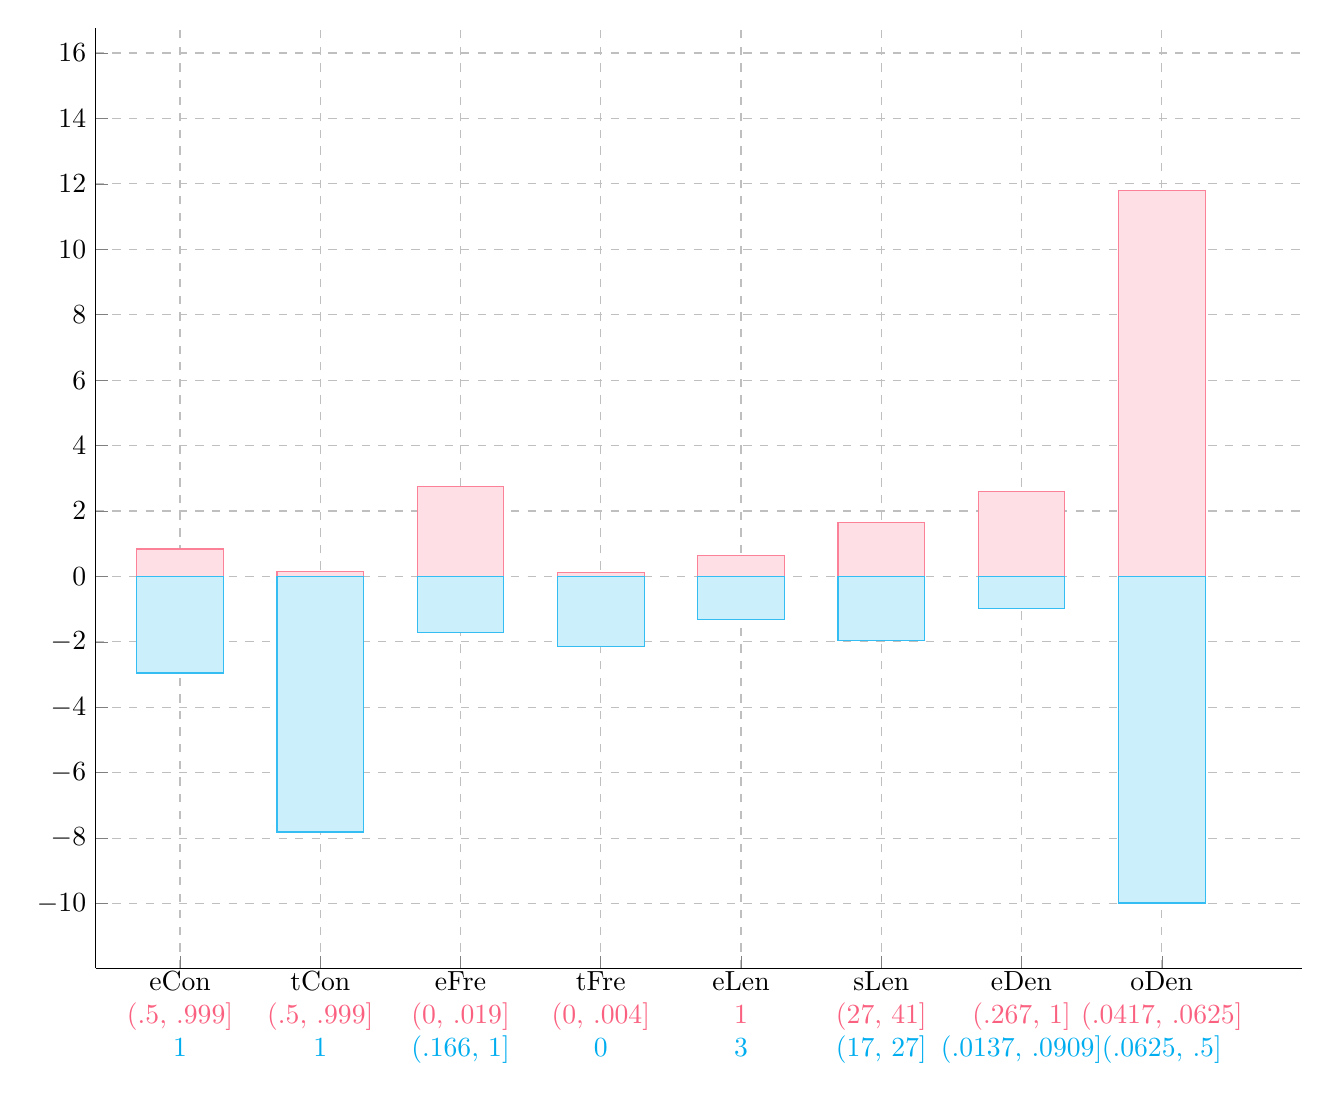
\begin{tikzpicture}
  \centering
  \begin{axis}[%ybar=1.0pt,
    ybar stacked,
    height=13.52cm,
    %width=16.9cm, % 12->9,  9->6.93,  8-> 6
    width=16.9cm, % 12->9,  9->6.93,  8-> 6
    bar width=1.1cm,
    xmin=0.4,
    xmax=9,
    ymin=-11.976,
    ymax=13.010000000000002,
    enlarge y limits={upper,value=0.15},
    axis lines*=left,
    legend style={at={(0.5,-0.25)},anchor=north,legend columns=-1,
    /tikz/every even column/.append style={column sep=0.2cm}},
    %xticklabels={\textcolor{brinkpink}{S}-\textcolor{aogreen}{L},\textcolor{brinkpink}{M}-\textcolor{aogreen}{S},\textcolor{brinkpink}{L}-\textcolor{aogreen}{M},\textcolor{brinkpink}{S}-\textcolor{aogreen}{S},\textcolor{brinkpink}{M}-\textcolor{aogreen}{M},\textcolor{brinkpink}{L}-\textcolor{aogreen}{L},\textcolor{brinkpink}{S}-\textcolor{aogreen}{S},\textcolor{brinkpink}{M}-\textcolor{aogreen}{M}},
    xticklabels={eCon \\ \textcolor{brinkpink}{(.5, .999]} \\ \textcolor{cyan}{1}, tCon \\ \textcolor{brinkpink}{(.5, .999]} \\ \textcolor{cyan}{1}, eFre \\ \textcolor{brinkpink}{(0, .019]} \\ \textcolor{cyan}{(.166, 1]}, tFre \\ \textcolor{brinkpink}{(0, .004]} \\ \textcolor{cyan}{0}, eLen \\ \textcolor{brinkpink}{1} \\ \textcolor{cyan}{3}, sLen \\ \textcolor{brinkpink}{(27, 41]} \\ \textcolor{cyan}{(17, 27]}, eDen \\ \textcolor{brinkpink}{(.267, 1]} \\ \textcolor{cyan}{(.0137, .0909]}, oDen \\ \textcolor{brinkpink}{(.0417, .0625]} \\ \textcolor{cyan}{(.0625, .5]}},
    xtick=data,
    xmajorgrids=true,
    ymajorgrids=true,
    zmajorgrids=true,
    grid style=dashed,
    xticklabel style={
        inner sep=1pt,
	align=center,
        %rotate=90,
        %anchor=near xticklabel,
    },
    ]
    %\addplot [draw=aogreen!80,fill=aogreen!20] table[x=id,y=y]{
    \addplot [draw=cyan!80,fill=cyan!20] table[x=id,y=y]{
    id  y
    	1	-2.95
	2	-7.81
	3	-1.71
	4	-2.14
	5	-1.32
	6	-1.96
	7	-0.97
	8	-9.98
    };
    \addplot [draw=brinkpink!80,fill=brinkpink!20] table[x=id,y=y]{
    id  y
    	1	0.84
	2	0.16
	3	2.75
	4	0.13
	5	0.63
	6	1.66
	7	2.59
	8	11.8
    };
  \end{axis}
\end{tikzpicture}

\end{document}

